% Chapter Template

\chapter{Experiments and results} % Main chapter title

\label{Chapter5} % Change X to a consecutive number; for referencing this chapter elsewhere, use \ref{ChapterX}

\lhead{Chapter 5. \emph{Experiments and results}} % Change X to a consecutive number; this is for the header on each page - perhaps a shortened title

After discussing how Crawl.js works we want to run some experiments. We decided to test Crawl.js in a closed environment. Crawling the public internet requires a good supervision and the required work to do that is simply out of scope of this thesis. All experiments were done on the Opennebula cluster hosted at the university of Neuchatel.
\\
First we describe our \emph{measurement} techniques and how our \emph{setup} looks like. The \emph{setup} will stay the same during all experiments but we will use different network topologies (achieved with virtual latencies) during our work. In \emph{experiment 1} we use a topology with one region (no latencies) to verify some basic properties of Crawl.js (e.g. scaling). In \emph{Experiment 2 \& 3} we introduce a new topology with 2 regions and focus on the \emph{closeness} aspect of Crawl.js.

\section{Measurement}
Throughout our experiments we use the unit pages/second to measure performance. We measure every worker independently, so the overall system performance is the sum of all measured worker performances. One worker measurement is done as follows:
\begin{itemize}
  \item We instrument how long it takes to crawl \emph{10'000 pages}
  \item Taking the arithmetic mean gives us \emph{pages/second} per worker
  \item Because we observed a big variance in our values we repeated one worker measurement several time and computed again the arithmetic mean.
\end{itemize}
Of course this unit depends highly on the worker hardware. Our numbers are base on a hardware configuration as detailed in Appendix~\ref{appendix:worker}

\section{Setup}
To do our experiments we had to setup the following types of VM in the cluster:
\begin{itemize}
\item www - static Wikipedia snapshots.
\item Redis - remote queues.
\item workers - crawls pages from \emph{www} and updates remote queues in \emph{Redis}.
\end{itemize}
All VM's are based on a ubuntu server 12.04.3 LTS (64bit) image.

To setup and manage (workers) the VMs efficiently we wrote some basic bash scripts. It allowed us to deploy different worker configurations easily and perform basic operations on the workers such as start and stop. Having those scripts saved us a lot of time throughout the different experiments we ran. You find all scripts used throughout our experiments in the Crawl.js git repository. In Figure~\ref{test_setup} is an overview of all the VMs used during the experiments.

\begin{figure}[h]
\centering
  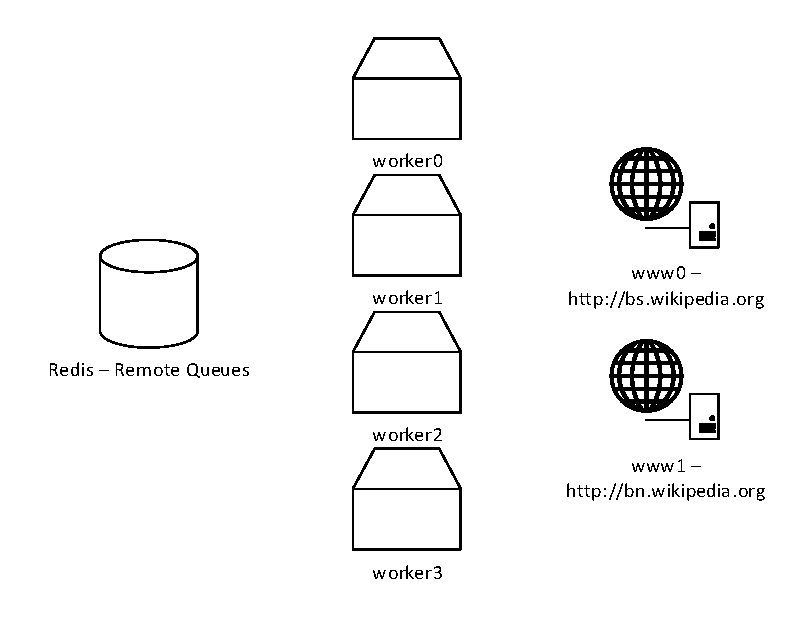
\includegraphics[width=1.0\textwidth]{Figures/experiments_setup.pdf}
\caption{Crawl.js - Test setup overview}
\label{test_setup}
\end{figure}

\subsection{www - Wikipedia snapshots}
In order to have realistic sites to crawl we decided to setup Wikipedia html dumps. Unfortunately their dumper stopped back in 2008 and therefore the snapshots are pretty old. But for our use case it is good enough. Back then, the different Wikipedia languages were located in different subdirectories but all on the same host. But we need links pointing to different servers to be able to add latency to some of the sites and experiment with the \emph{closeness} aspect of Crawl.js. Therefore we wrote an xsl transformation script to change all language links from /lang/index.html to lang.wikipedia.org/index.html.


Additionally we encountered a serious performance problem during our first tests. The random read performance in our VM was about 200 IOPS (tested with fio). Therefore the web server (nginx) could not deliver pages fast enough and represented the bottleneck in our setup. In order to circumvent this unwanted side effect we put our html dumps on a ram filesystem (tmpfs) and random read performance was not an issue anymore.

\begin{itemize}
  \item CPU: 1, VCPU: 1
  \item RAM: 2048M
\end{itemize}

\subsection{Redis - Remote queues}
During our experiments we ran a single Redis server instance. Because all the URLs have to fit in memory, setting up a Redis cluster to share the key space on different servers is inevitable as soon the number of URLs becomes too big. In our simple/small setup this was not needed. During our experiments we encountered 217'690 URLs which represents 82M of data inside the Redis server (Redis info command).

\begin{itemize}
  \item CPU: 1, VCPU: 1
  \item RAM: 3072M
\end{itemize}

\subsection{worker - Crawl.js worker instance}
The worker VM hosts our developed crawler (Crawl.js instance). Setting it up was straight forward. First we thought that we could host more than one crawler instance (using multiple cpus) but we achieved better results with one crawler per worker. This 1:1 worker to crawler relation made the management easier too.

\begin{itemize}
  \item CPU: 1, VCPU: 1
  \item RAM: 1024M
\end{itemize}

\subsection{Stores}
The reader may have noticed that this component is missing in our test setup. We intentionally left it out in order to reduce noise and focus on the performance impact of locality. We also wanted to verify a correct URL handling within the \emph{queues} in Redis. Disabling the \emph{store} component was a matter of changing a configuration value. In all our experiments we used the \emph{dummy} store implementation which does nothing but pipe the downloaded content to /dev/null.

\section{Experiment 1}

The goal of our first experiment was to verify the following basic properties of Crawl.js.

\begin{itemize}
  \item The crawl stops.
  \item Adding more workers improves the overall crawl performance. (scalability)
  \item All pages are found (starting with a single seed URL).
\end{itemize}

Therefore, we use a simple network topology with one region and no latencies as shown in Figure~\ref{topology_exp1}.

\begin{figure}[h]
\centering
  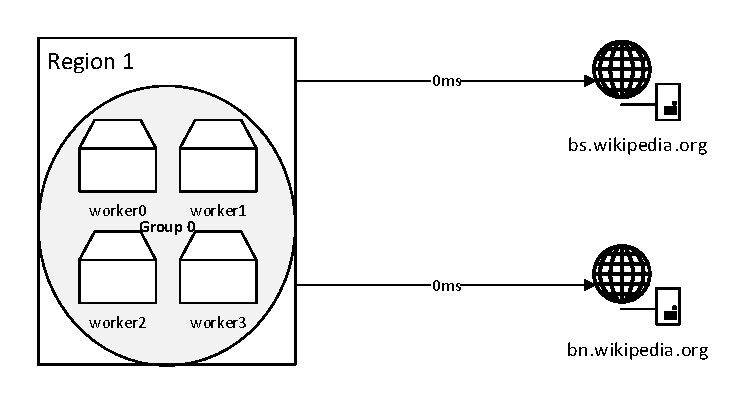
\includegraphics[width=1.0\textwidth]{Figures/topology_exp1.pdf}
  \caption{Network Topology: 1 region, 1 group (no additional virtual latencies)}
\label{topology_exp1}
\end{figure}

\subsection{Configuration}

Here, is an overview of the configuration we use.

\begin{itemize}
  \item Workers: 1, 2, 3, 4 \& 5
  \item Sites: http://bn.wikipedia.org, http://bs.wikipedia.org
  \item Topology: 1 region (no latencies) as shown in Figure~\ref{topology_exp1}
\end{itemize}

\subsection{Analysis}

All tests started with the same seed URL (http://bn.wikipedia.org). Verifying the first property \emph{the crawl stops} was straight forward and done manually. \emph{Adding more workers improves the overall crawl performance} was verified too, as shown in Figure~\ref{plot:exp_001}. The scaling behaviour actually exceeded our expectations as it was linear. We were able to add workers and observe a constant increase of the whole system performance. Doing this we also observed that the performance per worker reaches its maximum only in a system with at least 3 workers (\~260 pages/second). We tried to explain this behaviour with bandwidth limitations a single worker has (100mbit), but our assumptions turned out to be wrong and we still can not explain it. Hopefully, a system with less than 3 workers is rather uncommon and we decided to not further investigate in finding the bottleneck causing this behaviour.
\newline
\newline
For the last property \emph{All pages are found}, Wikipedia provides a downloadable text file containing all article URLs. Using this file we were able to import the expected URLs into Redis (set datastructure). Afterwards we took the difference (Redis diff) between the two sets 'urls:expected' and 'urls:crawled'. Unfortunately the resulting set was not empty. It had 23'338 URLs. That number seemed us pretty huge, thats about 16\% of all articles. We decided to have a closer look at some randomly picked articles to check what we actually missed. We discovered quickly that most of these 'missed' articles redirected (alias) to other articles we did crawl (13'391 redirect articles). Because articles never reference articles through an alias, Crawl.js did not discover those 'redirect-articles' (as we follow references,<a> tags). This still leaves us with 9'947 (7\%) of potentially missed articles. Again we randomly picked some of the remaining articles and discovered that none of them were referenced by other articles (using grep -r). Of course we did not check for references to all remaining articles but 7\% of orphaned articles~\footnote{\url{http://en.wikipedia.org/wiki/Wikipedia:WikiProject_Orphanage}} seemed us realistic and therefore the verification of this property good enough to proceed with our experiments.
\newline
\newline
\begin{figure}
\centering
  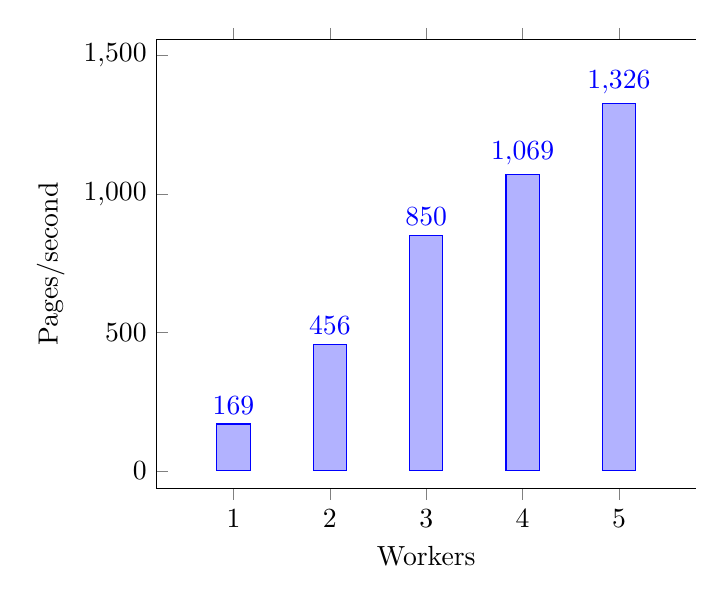
\begin{tikzpicture} 
    \begin{axis}[
      ybar,
      bar width=12pt,
      enlargelimits=0.2,
      axis y line*=left,
      xlabel={Workers},
      xlabel near ticks,
      ylabel={Pages/second},
      ylabel near ticks,
      xtick=data,
      nodes near coords,
      nodes near coords align={vertical},
      ]
      \addplot
        coordinates {(1,169) (2,456) (3,850) (4,1069) (5,1326)};
    \end{axis}
  \end{tikzpicture}
\caption{Scaling behaviour (1, 2, 3, 4 \& 5 workers)}
\label{plot:exp_001}
\end{figure}

\section{Experiment 2}

In this experiment we took the same components (4 workers) as in experiment 1 but we introduced a new network topology with 2 regions as shown in Figure~\ref{topology_exp2}. Basically, we introduced two virtual regions by adding latencies between workers and Wikipedia servers. The latency values used reflect the \emph{closeness} of the regions towards the Wikipedia servers. With this new topology we want to demonstrate how drastically crawl performance suffers when dealing with latencies. Especially when using a random URL to worker assignment. In experiment 3 we will reconfigure the system in order to obtain better crawl performances with the same network topology in place.

\begin{figure}[h]
\centering
  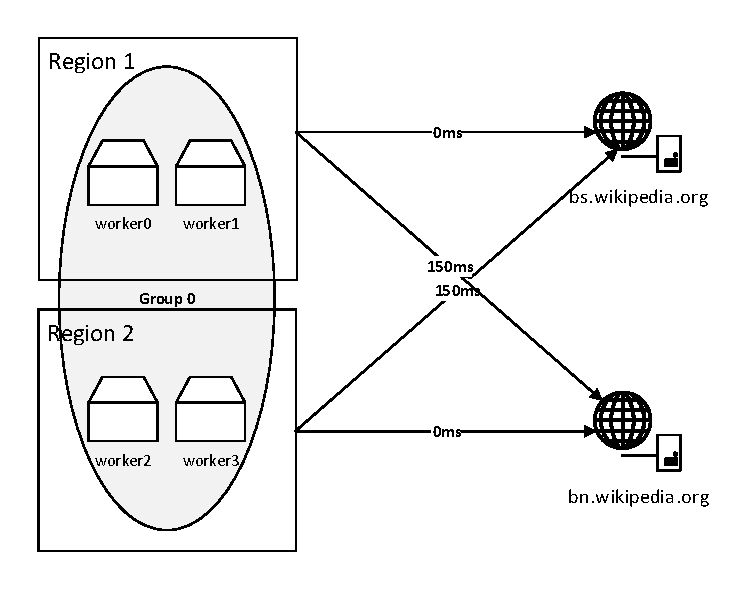
\includegraphics[width=1.0\textwidth]{Figures/topology_exp2.pdf}
  \caption{Network Topology: 2 regions, 1 group (with additional latencies)}
\label{topology_exp2}
\end{figure}

\subsection{Configuration}
\begin{itemize}
  \item Groups:
    \begin{itemize}
      \item Config 0: 1 group with 4 blocks
    \end{itemize}
  \item Workers: 4
  \item Sites: http://bs.wikipedia.org, http://bn.wikipedia.org
  \item Topologies: 1 region (Figure~\ref{topology_exp1}) and 2 regions (Figure~\ref{topology_exp2})
\end{itemize}

\subsection{Analysis}
Exactly as in experiment 1 all tests started with a single seed URL. Figure~\ref{plot:exp_002} shows our measured performances, once for a network topology without additional latencies (from experiment 1) and once for the new network topology with additional latencies (2 regions). As one can see in Figure~\ref{plot:exp_002}, the performance difference is huge. Crawling on the second network topology is 4 times worse. Based on the latencies we added this observation can be explained as follows:
\\
\\
Because we fetch many pages in parallel we first need to break down the performance to one connection:
\[ 
  P_c = \frac{P}{n_w n_c}
\]
\begin{tabular}{@{}>{$}l<{$}l@{}}
  n_w & Number of workers\\
  n_c & Concurrent connections per worker\\
  P & Measured overall performance\\
P_c & Performance per connection\\
\end{tabular}

\begin{itemize}
  \item $ P1_c $ is the performance per connection for topology 1, $ P2_c $ for topology 2 
  \item $ P1_c = 22.15 $ pages/second ($ n_w = 4, n_c = 10, P = 886 $) 
  \item $ P2_c = 5.25 $ pages/second ($ n_w = 4, n_c = 10, P = 210 $)
\end{itemize}
Of course $ \frac{1}{P_c} $ is the time we need to crawl one page:
\begin{itemize}
  \item $ \frac{1}{P1_c} = \frac{1}{22.15} $ seconds/page
  \item $ \frac{1}{P2_c} = \frac{1}{5.25} $ seconds/page
\end{itemize}

So, intuitively the difference $ \frac{1}{P2_c} - \frac{1}{P1_c} $ should roughly be equal to expected mean latency.
\[ \frac{1}{5.25} - \frac{1}{22.15} \approx  0.145\]

Our expected mean latency is $ \approx 0.075s $, assuming that the number of pages on both sites is equal. So why do we still miss an additional $ \approx 0.07s $. More precisely a factor 2. In order to explain that we need to have a look at the following \emph{tcpdump} extract made on an average\footnote{Average in terms of size. Larger pages have a higher-, smaller pages a lower total latency. Therefore we use an average page size as an approximation} page.

\begin{lstlisting}[language=bash]
#page size: 14607 bytes, latency: 100ms

duration: 0.100 + 0.402 = 0.502s

handshake: 0.200s
17:38:31.477105 IP 192.168.98.9.59418 > 192.168.98.16.http: ...
17:38:31.477137 IP 192.168.98.16.http > 192.168.98.9.59418: ...
17:38:31.577468 IP 192.168.98.9.59418 > 192.168.98.16.http: ...

payload: 0.200s
17:38:31.577924 IP 192.168.98.9.59418 > 192.168.98.16.http: ...
...
17:38:31.779264 IP 192.168.98.9.59418 > 192.168.98.16.http: ...

close: 0.100s
17:38:31.779489 IP 192.168.98.9.59418 > 192.168.98.16.http: ...
17:38:31.779539 IP 192.168.98.16.http > 192.168.98.9.59418: ...
17:38:31.879843 IP 192.168.98.9.59418 > 192.168.98.16.http: ...
\end{lstlisting}

As you can see adding 100ms (same goes for 150ms) of latency results in a total duration of 0.502s. So in a scenario where we open and close a tcp connection for each page we need to consider a factor 5 between added latency and effective duration on this average page. But in our above logical consequences we need a factor 2. Hopefully, Crawl.js keeps sockets open and therefore handshaking/closing the connection is done once only.\footnote{In real world things are even more complicated (several handshaking/closing) because we fetch from different sites simultaneously.}. So removing those phases results in a total duration of $ \approx 0.200s $ which is twice (factor 2) as long as our added latency. And our above logics are valid.

\begin{figure}
  \centering
  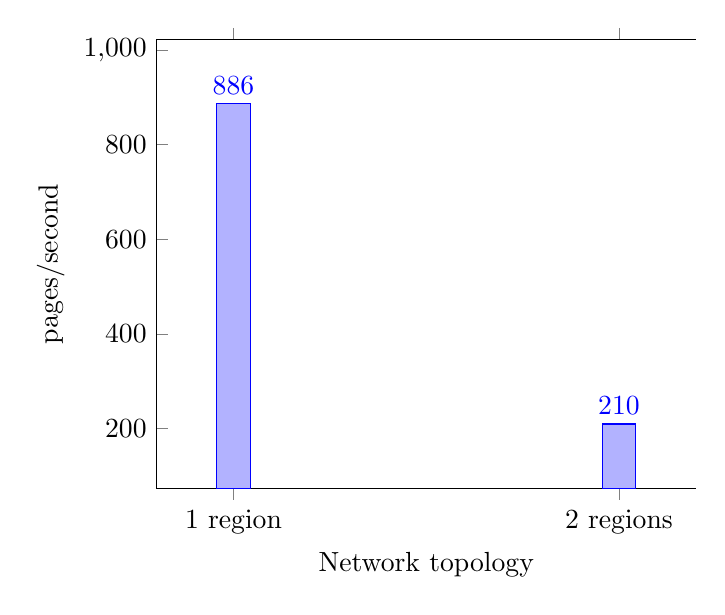
\begin{tikzpicture} 
    \begin{axis}[
        ybar,
        bar width=12pt,
        axis y line*=left,
        enlargelimits=0.2,
        xlabel={Network topology},
        symbolic x coords={1 region, 2 regions},
        xlabel near ticks,
        ylabel={pages/second},
        ylabel near ticks,
        xtick=data,
        nodes near coords,
        nodes near coords align={vertical},
      ]
      \addplot
      coordinates {(1 region, 886) (2 regions,210)};
    \end{axis}
  \end{tikzpicture}
  \caption{Crawl performance on different network topologies}
  \label{plot:exp_002}
\end{figure}

\section{Experiment 3}

In the previous experiment we showed that latency on sites affect the crawl performance heavily. In this experiment we want to demonstrate that Crawl.js is able to deal with different latencies on different sites. We want to show that when using the same topology as in experiment 2 we are able to achieve better performance by reconfiguring Crawl.js. We will keep the number of workers the same but we will regroup them differently in order to respect \emph{closeness}. Figure~\ref{topology_exp3} shows how we grouped the workers. 

\subsection{Configuration}
In experiment 2 we had only one group and the URL to worker assignment was done randomly. The result was that every worker was affected by the latency. So in order to achieve a better performance we need to avoid cross-region crawls. Therefore we introduce a second group and each group will be assigned to one site only. Group 0 for bs.wikipedia.org and group 1 for bn.wikipedia.org. With this setup workers won't be affected anymore by the cross-region latencies which should result in better crawl performance. Figure~\ref{plot:exp_003} shows our measurements.
\\
The configuration used is as follows:
\begin{itemize}
  \item Workers: 4
  \item Groups:
    \begin{itemize}
      \item Config 0: 1 group with 4 blocks (as in experiment 2)
      \item Config 1: 2 groups with 2 blocks each (as shown in Figure~\ref{topology_exp3})
    \end{itemize}
  \item Sites: http://bs.wikipedia.org, http://bn.wikipedia.org
  \item Topology: 2 regions (Figure~\ref{topology_exp3})
\end{itemize}

\subsection{Analysis}

Figure~\ref{plot:exp_003} shows two measurements: the previous value from experiment 2 and the new value from this experiment. As you can see we were able to improve the crawl performance heavily. A simple reconfiguration made all workers crawl latency-free sites only and this in turn resulted in a performance almost as good as measured in experiment 1 (1 region, no additional latencies). This fact clearly demonstrates that Crawl.js can be configured in such a way that \emph{closeness} to sites is respected.
\begin{figure}
  \centering
  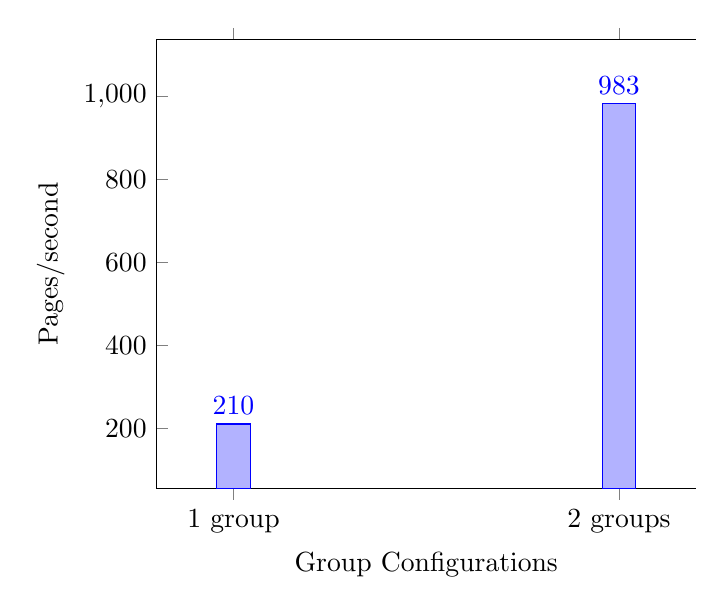
\begin{tikzpicture} 
    \begin{axis}[
        ybar,
        bar width=12pt,
        axis y line*=left,
        enlargelimits=0.2,
        xlabel={Group Configurations},
        symbolic x coords={1 group, 2 groups},
        xlabel near ticks,
        ylabel={Pages/second},
        ylabel near ticks,
        xtick=data,
        nodes near coords,
        nodes near coords align={vertical},
      ]
      \addplot
      coordinates {(1 group,210) (2 groups,983)};
    \end{axis}
  \end{tikzpicture}
  \caption{Crawl performance using different group configurations (on 2 regions)}
  \label{plot:exp_003}
\end{figure}

\begin{figure}[h]
\centering
  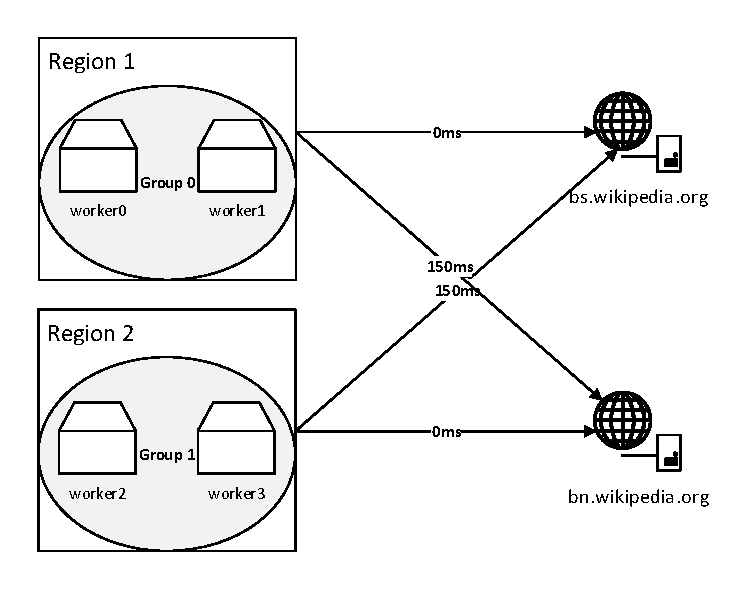
\includegraphics[width=1.0\textwidth]{Figures/topology_exp3.pdf}
  \caption{Network Topology: 2 regions, 2 groups (with latencies)}
\label{topology_exp3}
\end{figure}
